\documentclass[10pt]{article}

\usepackage[margin=0.55in]{geometry}
\usepackage{graphicx}
\usepackage{caption}
\usepackage{tikz}
\usetikzlibrary{arrows.meta, positioning, fit, backgrounds}

\pagestyle{plain}

\tikzset{
  box/.style={
    rectangle,
    rounded corners,
    draw,
    align=center,
    minimum height=8mm,
    text width=31mm,
    font=\scriptsize
  },
  smallbox/.style={
    rectangle,
    rounded corners,
    draw,
    align=center,
    minimum height=7mm,
    text width=27mm,
    font=\scriptsize
  },
  group/.style={
    rectangle,
    rounded corners,
    draw,
    dashed,
    inner sep=6pt
  },
  arrow/.style={-{Latex[length=2mm]}, thick},
  dataarrow/.style={-{Latex[length=2mm]}, thick, dashed},
  note/.style={font=\scriptsize, align=center}
}

\begin{document}

\begin{center}
{\Large Engkanto Clash Architecture Diagrams}
\end{center}

\section*{1. High-Level Architecture}

\begin{center}
\resizebox{\textwidth}{!}{%
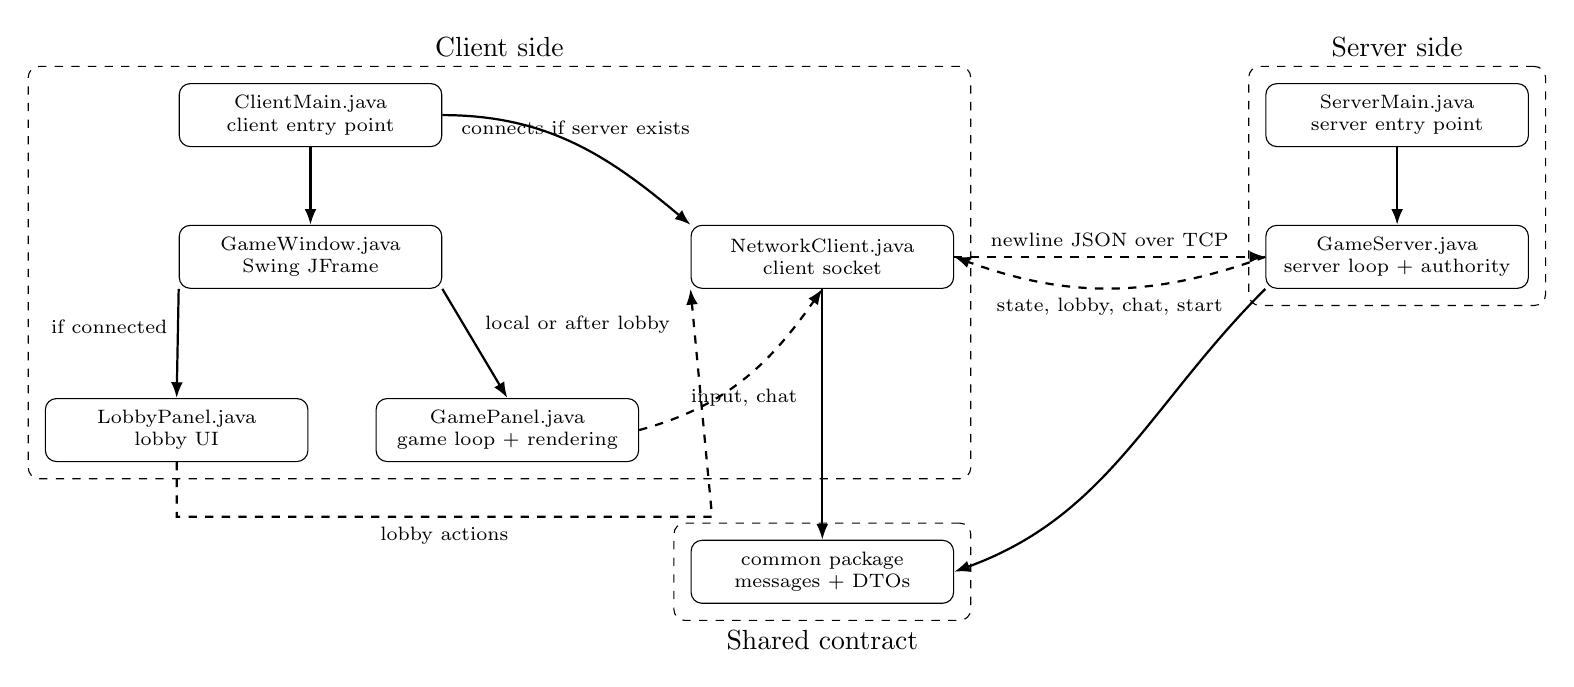
\begin{tikzpicture}[x=1cm,y=1cm]
\node[box] (clientmain) at (2.5,7.1) {ClientMain.java\\client entry point};
\node[box] (window) at (2.5,5.3) {GameWindow.java\\Swing JFrame};
\node[box] (lobby) at (0.8,3.1) {LobbyPanel.java\\lobby UI};
\node[box] (gamepanel) at (5.0,3.1) {GamePanel.java\\game loop + rendering};
\node[box] (netclient) at (9.0,5.3) {NetworkClient.java\\client socket};
\node[box] (common) at (9.0,1.3) {common package\\messages + DTOs};
\node[box] (servermain) at (16.3,7.1) {ServerMain.java\\server entry point};
\node[box] (server) at (16.3,5.3) {GameServer.java\\server loop + authority};

\draw[arrow] (clientmain) -- (window);
\draw[arrow] (window.south west) -- node[note, above left] {if connected} (lobby.north);
\draw[arrow] (window.south east) -- node[note, above right] {local or after lobby} (gamepanel.north);
\draw[arrow] (clientmain.east) to[out=0,in=140] node[note, above] {connects if server exists} (netclient.north west);
\draw[arrow] (servermain) -- (server);
\draw[dataarrow] (lobby.south) -- (0.8,2.0) -- node[note, below] {lobby actions} (7.6,2.0) -- (netclient.south west);
\draw[dataarrow] (gamepanel.east) to[out=15,in=235] node[note, below] {input, chat} (netclient.south);
\draw[dataarrow] (netclient.east) -- node[note, above] {newline JSON over TCP} (server.west);
\draw[dataarrow] (server.west) to[out=200,in=-20] node[note, below] {state, lobby, chat, start} (netclient.east);
\draw[arrow] (netclient.south) -- (common.north);
\draw[arrow] (server.south west) to[out=-135,in=20] (common.east);

\node[group, fit=(clientmain)(window)(lobby)(gamepanel)(netclient), label=above:Client side] {};
\node[group, fit=(servermain)(server), label=above:Server side] {};
\node[group, fit=(common), label=below:Shared contract] {};
\end{tikzpicture}%
}
\captionof{figure}{High-level architecture of Engkanto Clash.}
\end{center}

\clearpage
\section*{2. Multiplayer Gameplay Message Flow}

\begin{center}
\resizebox{\textwidth}{!}{%
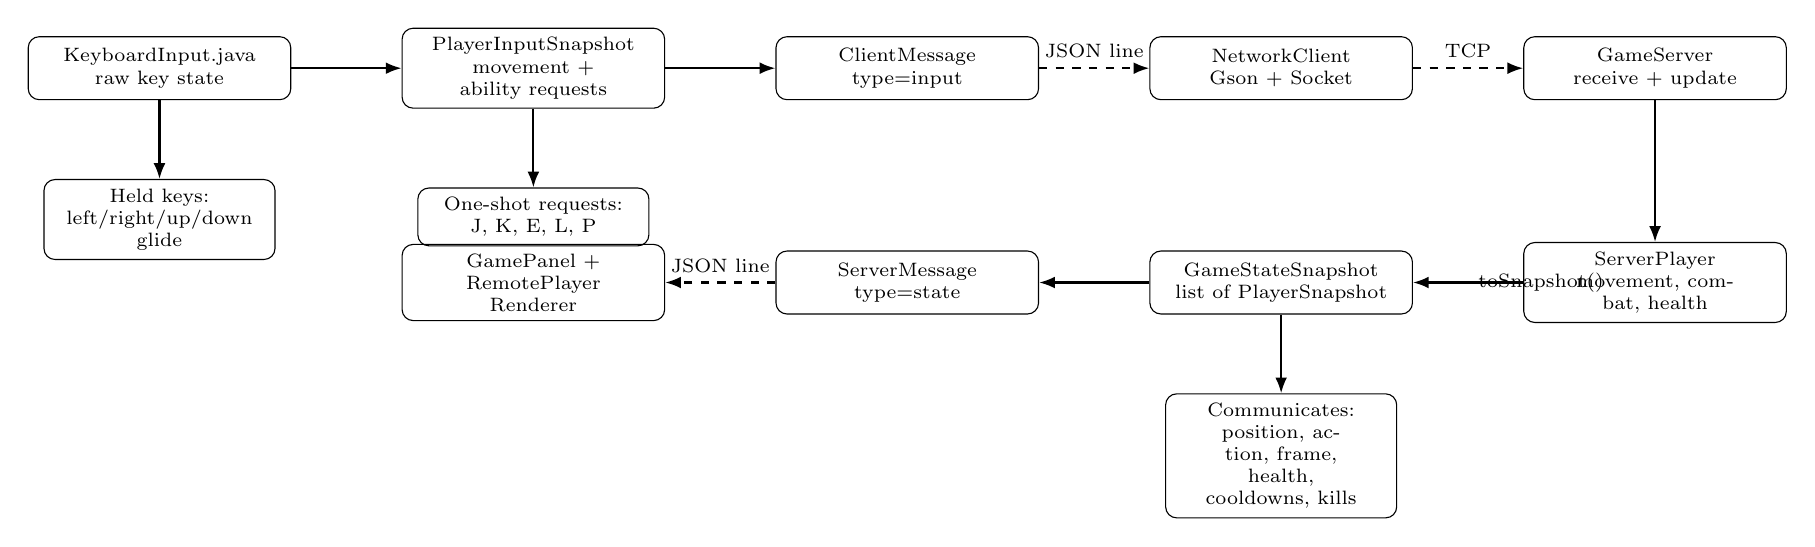
\begin{tikzpicture}[node distance=10mm and 14mm]
\node[box] (keyboard) {KeyboardInput.java\\raw key state};
\node[box, right=of keyboard] (inputdto) {PlayerInputSnapshot\\movement + ability requests};
\node[box, right=of inputdto] (clientmsg) {ClientMessage\\type=input};
\node[box, right=of clientmsg] (netclient) {NetworkClient\\Gson + Socket};
\node[box, right=of netclient] (gameserver) {GameServer\\receive + update};
\node[box, below=18mm of gameserver] (serverplayer) {ServerPlayer\\movement, combat, health};
\node[box, left=of serverplayer] (gamestate) {GameStateSnapshot\\list of PlayerSnapshot};
\node[box, left=of gamestate] (servermsg) {ServerMessage\\type=state};
\node[box, left=of servermsg] (renderer) {GamePanel +\\RemotePlayer\\Renderer};
\node[smallbox, below=of keyboard] (held) {Held keys:\\left/right/up/down\\glide};
\node[smallbox, below=of inputdto] (oneshot) {One-shot requests:\\J, K, E, L, P};
\node[smallbox, below=of gamestate] (statecontains) {Communicates:\\position, action, frame,\\health, cooldowns, kills};

\draw[arrow] (keyboard) -- (inputdto);
\draw[arrow] (inputdto) -- (clientmsg);
\draw[dataarrow] (clientmsg) -- node[note, above] {JSON line} (netclient);
\draw[dataarrow] (netclient) -- node[note, above] {TCP} (gameserver);
\draw[arrow] (gameserver) -- (serverplayer);
\draw[arrow] (serverplayer) -- node[note, right] {toSnapshot()} (gamestate);
\draw[arrow] (gamestate) -- (servermsg);
\draw[dataarrow] (servermsg) -- node[note, above] {JSON line} (renderer);
\draw[arrow] (keyboard) -- (held);
\draw[arrow] (inputdto) -- (oneshot);
\draw[arrow] (gamestate) -- (statecontains);
\end{tikzpicture}%
}
\captionof{figure}{Client input is sent to the server; server snapshots are rendered by the client.}
\end{center}

\clearpage
\section*{3. Lobby And Chat Communication}

\begin{center}
\resizebox{\textwidth}{!}{%
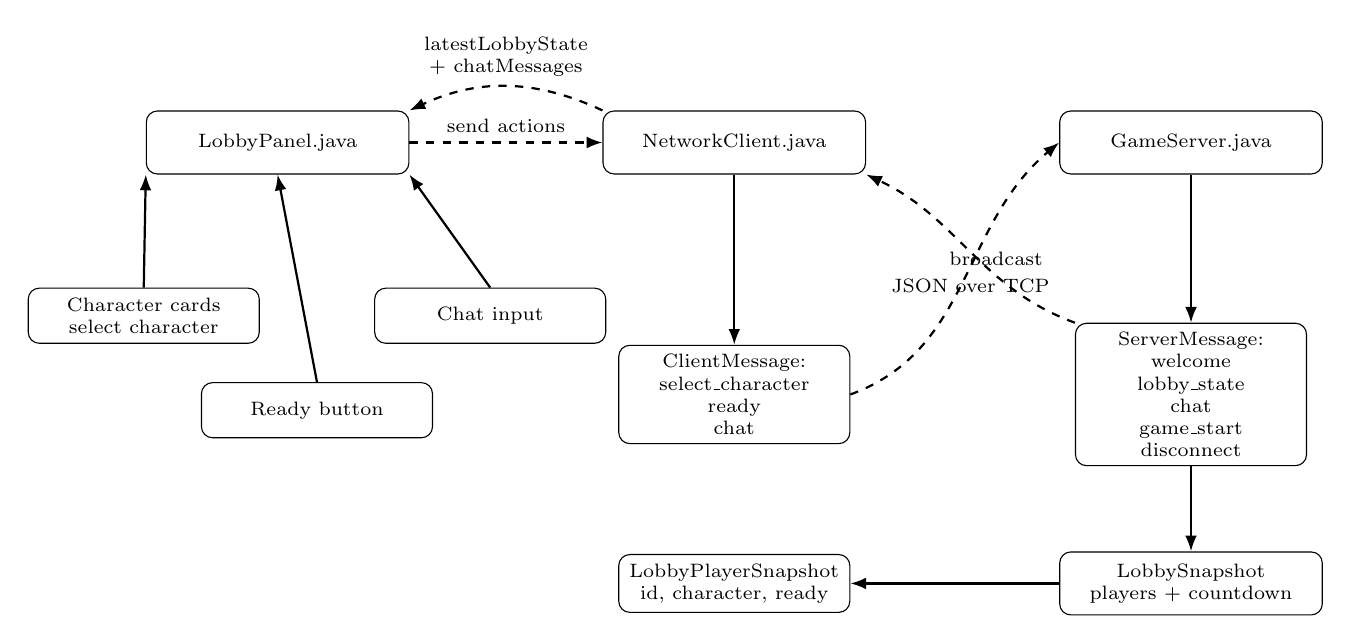
\begin{tikzpicture}[x=1cm,y=1cm]
\node[box] (lobby) at (2.4,6.4) {LobbyPanel.java};
\node[box] (netclient) at (8.2,6.4) {NetworkClient.java};
\node[box] (server) at (14.0,6.4) {GameServer.java};
\node[smallbox] (select) at (0.7,4.2) {Character cards\\select character};
\node[smallbox] (ready) at (2.9,3.0) {Ready button};
\node[smallbox] (chatui) at (5.1,4.2) {Chat input};
\node[smallbox] (clientmsgs) at (8.2,3.2) {ClientMessage:\\select\_character\\ready\\chat};
\node[smallbox] (servermsgs) at (14.0,3.2) {ServerMessage:\\welcome\\lobby\_state\\chat\\game\_start\\disconnect};
\node[box] (lobbysnap) at (14.0,0.8) {LobbySnapshot\\players + countdown};
\node[smallbox] (lobbyplayer) at (8.2,0.8) {LobbyPlayerSnapshot\\id, character, ready};

\draw[arrow] (select.north) -- (lobby.south west);
\draw[arrow] (ready.north) -- (lobby.south);
\draw[arrow] (chatui.north) -- (lobby.south east);
\draw[dataarrow] (lobby.east) -- node[note, above] {send actions} (netclient.west);
\draw[arrow] (netclient.south) -- (clientmsgs.north);
\draw[dataarrow] (clientmsgs.east) to[out=20,in=220] node[note, below, pos=0.55] {JSON over TCP} (server.west);
\draw[arrow] (server.south) -- (servermsgs.north);
\draw[arrow] (servermsgs.south) -- (lobbysnap.north);
\draw[arrow] (lobbysnap.west) -- (lobbyplayer.east);
\draw[dataarrow] (servermsgs.north west) to[out=160,in=-25] node[note, above, pos=0.35] {broadcast} (netclient.south east);
\draw[dataarrow] (netclient.north west) to[out=155,in=25] node[note, above] {latestLobbyState\\+ chatMessages} (lobby.north east);
\end{tikzpicture}%
}
\captionof{figure}{Lobby and chat messages synchronize character selection, readiness, countdown, and chat.}
\end{center}

\clearpage
\section*{4. Server-Side Responsibilities}

\begin{center}
\resizebox{\textwidth}{!}{%
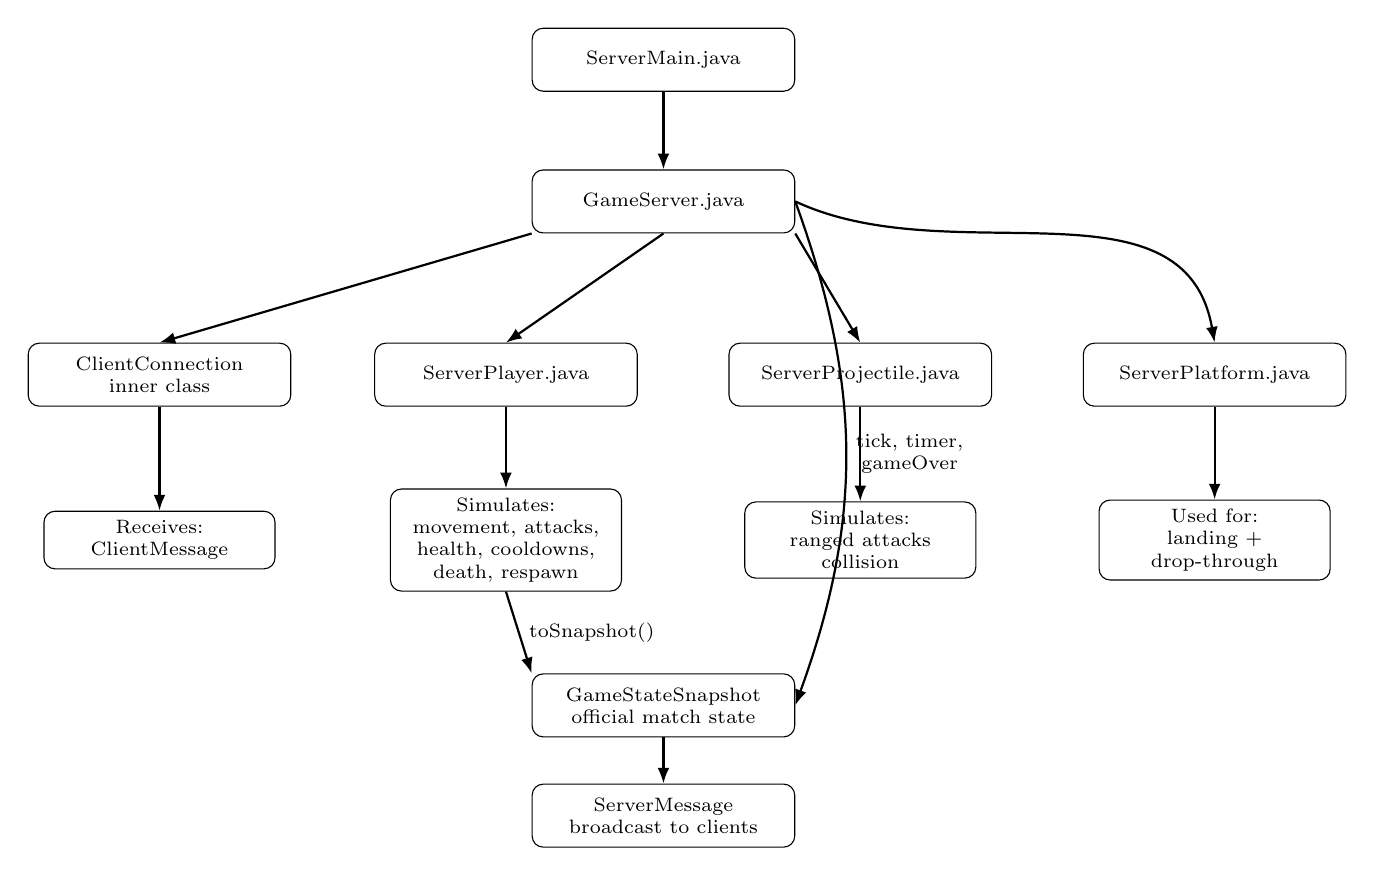
\begin{tikzpicture}[x=1cm,y=1cm]
\node[box] (servermain) at (8.0,9.8) {ServerMain.java};
\node[box] (gameserver) at (8.0,8.0) {GameServer.java};
\node[box] (connections) at (1.6,5.8) {ClientConnection\\inner class};
\node[box] (serverplayer) at (6.0,5.8) {ServerPlayer.java};
\node[box] (projectile) at (10.5,5.8) {ServerProjectile.java};
\node[box] (platform) at (15.0,5.8) {ServerPlatform.java};
\node[smallbox] (clientmsg) at (1.6,3.7) {Receives:\\ClientMessage};
\node[smallbox] (logic) at (6.0,3.7) {Simulates:\\movement, attacks,\\health, cooldowns,\\death, respawn};
\node[smallbox] (projlogic) at (10.5,3.7) {Simulates:\\ranged attacks\\collision};
\node[smallbox] (collision) at (15.0,3.7) {Used for:\\landing + drop-through};
\node[box] (snapshot) at (8.0,1.6) {GameStateSnapshot\\official match state};
\node[box] (servermsg) at (8.0,0.2) {ServerMessage\\broadcast to clients};

\draw[arrow] (servermain) -- (gameserver);
\draw[arrow] (gameserver.south west) -- (connections.north);
\draw[arrow] (gameserver.south) -- (serverplayer.north);
\draw[arrow] (gameserver.south east) -- (projectile.north);
\draw[arrow] (gameserver.east) to[out=-25,in=100] (platform.north);
\draw[arrow] (connections) -- (clientmsg);
\draw[arrow] (serverplayer) -- (logic);
\draw[arrow] (projectile) -- (projlogic);
\draw[arrow] (platform) -- (collision);
\draw[arrow] (logic.south) -- node[note, right] {toSnapshot()} (snapshot.north west);
\draw[arrow] (gameserver.east) to[out=-70,in=70] node[note, right] {tick, timer,\\gameOver} (snapshot.east);
\draw[arrow] (snapshot) -- (servermsg);
\end{tikzpicture}%
}
\captionof{figure}{The server owns multiplayer authority and broadcasts official state.}
\end{center}

\clearpage
\section*{5. Client Gameplay Rendering}

\begin{center}
\resizebox{\textwidth}{!}{%
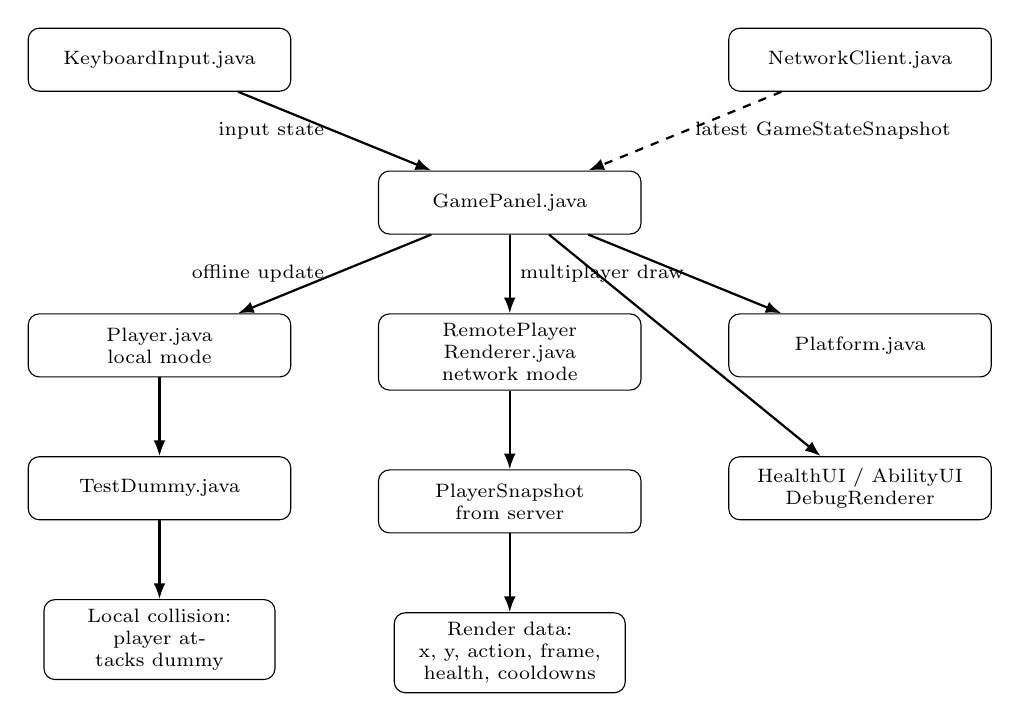
\begin{tikzpicture}[node distance=10mm and 11mm]
\node[box] (gamepanel) {GamePanel.java};
\node[box, above left=of gamepanel] (keyboard) {KeyboardInput.java};
\node[box, above right=of gamepanel] (netclient) {NetworkClient.java};
\node[box, below left=of gamepanel] (localplayer) {Player.java\\local mode};
\node[box, below=of gamepanel] (remote) {RemotePlayer\\Renderer.java\\network mode};
\node[box, below right=of gamepanel] (platform) {Platform.java};
\node[box, below=of localplayer] (dummy) {TestDummy.java};
\node[box, below=of remote] (snapshot) {PlayerSnapshot\\from server};
\node[box, below=of platform] (ui) {HealthUI / AbilityUI\\DebugRenderer};
\node[smallbox, below=of dummy] (localcombat) {Local collision:\\player attacks dummy};
\node[smallbox, below=of snapshot] (renderdata) {Render data:\\x, y, action, frame,\\health, cooldowns};

\draw[arrow] (keyboard) -- node[note, left] {input state} (gamepanel);
\draw[dataarrow] (netclient) -- node[note, right] {latest GameStateSnapshot} (gamepanel);
\draw[arrow] (gamepanel) -- node[note, left] {offline update} (localplayer);
\draw[arrow] (gamepanel) -- node[note, right] {multiplayer draw} (remote);
\draw[arrow] (gamepanel) -- (platform);
\draw[arrow] (gamepanel) -- (ui);
\draw[arrow] (localplayer) -- (dummy);
\draw[arrow] (dummy) -- (localcombat);
\draw[arrow] (remote) -- (snapshot);
\draw[arrow] (snapshot) -- (renderdata);
\end{tikzpicture}%
}
\captionof{figure}{GamePanel switches between local simulation and multiplayer snapshot rendering.}
\end{center}

\clearpage
\section*{6. Local Character And Combat Structure}

\begin{center}
\resizebox{\textwidth}{!}{%
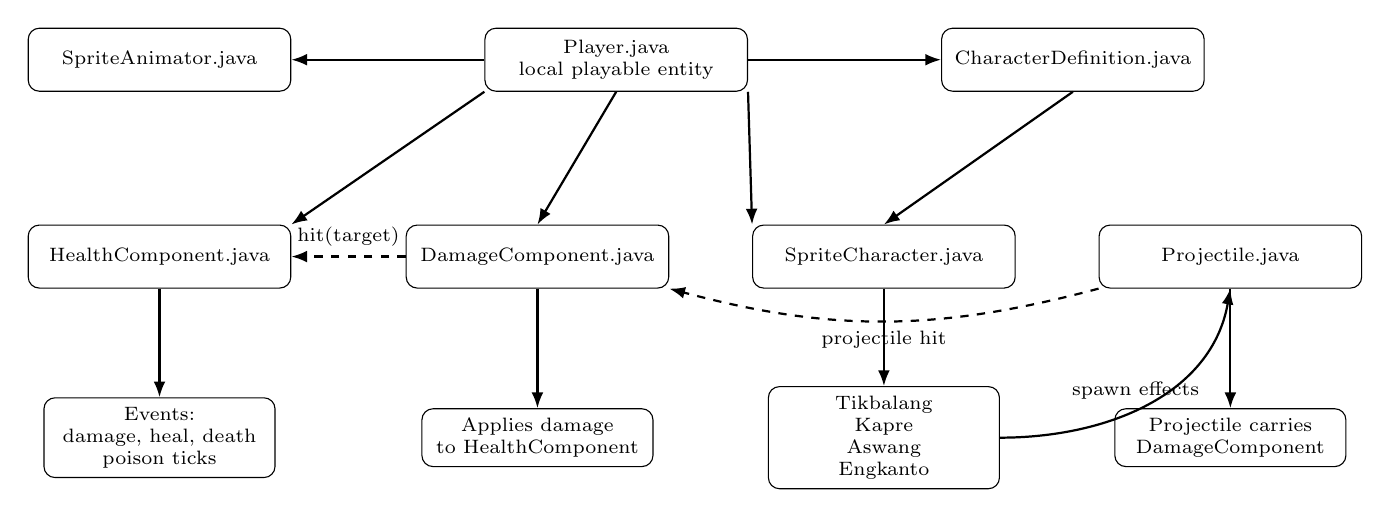
\begin{tikzpicture}[x=1cm,y=1cm]
\node[box] (animator) at (1.4,6.6) {SpriteAnimator.java};
\node[box] (player) at (7.2,6.6) {Player.java\\local playable entity};
\node[box] (interface) at (13.0,6.6) {CharacterDefinition.java};
\node[box] (health) at (1.4,4.1) {HealthComponent.java};
\node[box] (damage) at (6.2,4.1) {DamageComponent.java};
\node[box] (spritechar) at (10.6,4.1) {SpriteCharacter.java};
\node[box] (projectile) at (15.0,4.1) {Projectile.java};
\node[smallbox] (healthevents) at (1.4,1.8) {Events:\\damage, heal, death\\poison ticks};
\node[smallbox] (damageflow) at (6.2,1.8) {Applies damage\\to HealthComponent};
\node[smallbox] (characters) at (10.6,1.8) {Tikbalang\\Kapre\\Aswang\\Engkanto};
\node[smallbox] (projflow) at (15.0,1.8) {Projectile carries\\DamageComponent};

\draw[arrow] (player.west) -- (animator.east);
\draw[arrow] (player.east) -- (interface.west);
\draw[arrow] (interface.south) -- (spritechar.north);
\draw[arrow] (spritechar.south) -- (characters.north);
\draw[arrow] (player.south west) -- (health.north east);
\draw[arrow] (player.south) -- (damage.north);
\draw[arrow] (player.south east) -- (spritechar.north west);
\draw[arrow] (characters.east) to[out=0,in=-100] node[note, above, pos=0.45] {spawn effects} (projectile.south);
\draw[arrow] (health) -- (healthevents);
\draw[arrow] (damage) -- (damageflow);
\draw[arrow] (projectile) -- (projflow);
\draw[dataarrow] (damage.west) -- node[note, above] {hit(target)} (health.east);
\draw[dataarrow] (projectile.south west) to[out=-165,in=-15] node[note, below, pos=0.5] {projectile hit} (damage.south east);
\end{tikzpicture}%
}
\captionof{figure}{Local combat uses character definitions, animation, damage, health, and projectiles.}
\end{center}

\clearpage
\section*{7. One-Sentence Mental Model}

\begin{center}
\fbox{\parbox{0.9\textwidth}{
\centering
Clients send intent. The server sends truth. Shared DTOs define the contract. Rendering turns snapshots into visuals.
}}
\end{center}

\end{document}
